\chapter{Theory}
\label{theory}
%needs more references%
\section{Neural networks}
\label{theory}
To first begin, building these convolutional neural networks,  we must understand what a neural network is.
A neural network is a network of artificial neurons.
These neurons are sometimes referred to as perceptrons.
A perceptron takes in an input $x_i$ and uses trainable weights $w_i$, a bias $b$ and a given activation function to predict the expected output $y_i$.
Figure \ref{fig:neuron} provides an image representing a neuron. The activation functions commonly used include 

\begin{equation}
g(z) = \frac{1}{1+ exp(-z)}
 \qquad \text{Sigmoid function}
\end{equation}

\begin{equation}
g(z) = max(0,z)
 \qquad \text{Rectified Linear Unit(RELU) function}
\end{equation}

\begin{equation}
g(z) = \frac{exp(z)-exp(-z)}{exp(z) + exp(-z)}
 \qquad \text{Hyperbolic tangent function(Tanh)}
\end{equation}

\begin{equation}
g(\mathbf{z}) = \frac{exp(z_i)}{\sum_{j=1}^{K}exp(z_j)} \textrm{ for } i = 1,...,K \textrm{ and } \mathbf{z} = \{ z_1,....,z_K \} \in \mathbb{R}^K
 \qquad \text{Softmax}
\end{equation}

\begin{figure}
\centering
  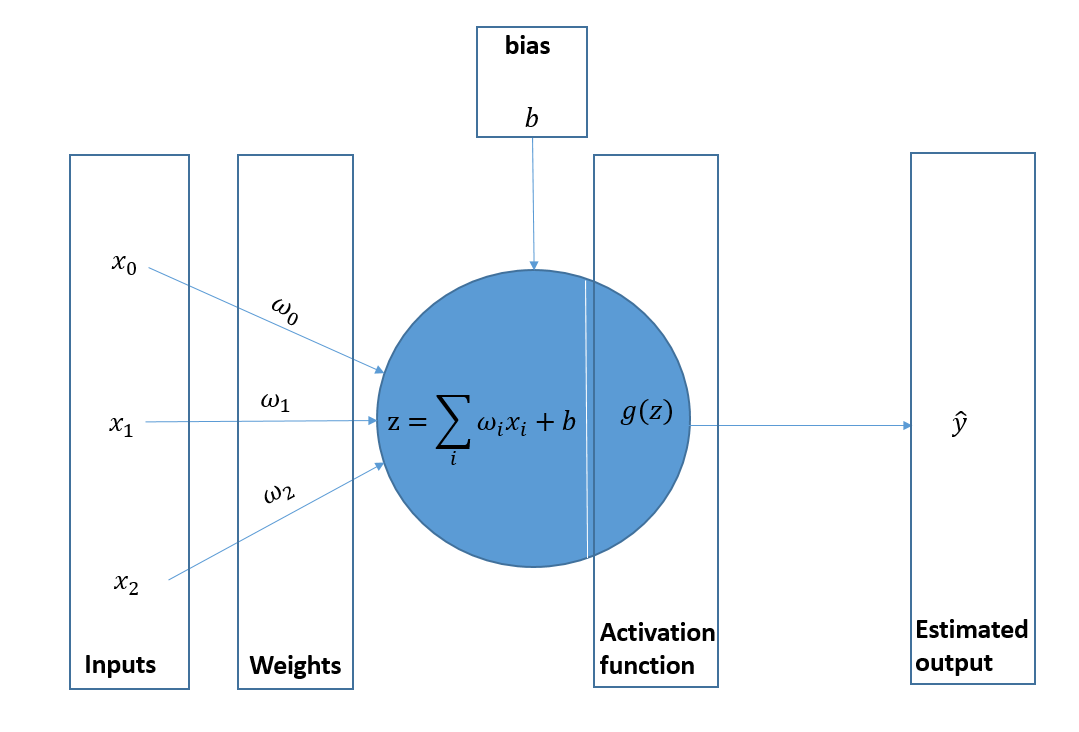
\includegraphics[width=75mm,scale=0.75]{neuron.PNG}
  \caption{Neuron}
  \label{fig:neuron}
\end{figure}

%todo stats around these activation functions.
Figure \ref{fig:activations} shows the plot of the sigmoid, RELU and Tanh activation functions. The sigmoid function gives an output between [0,1]. The RELU function also gives an output between [0,1], but it gives an output of 0 for inputs less than 0.  While the Tanh function gives an output between [-1,1].  The sigmoid function is usually used for binary classification while the softmax activation function is usually used for multi-class classification.  This is because the softmax function calculates the probabilities distribution of the output class $z_i$  over the different possible output classes.
\begin{figure}
\centering
  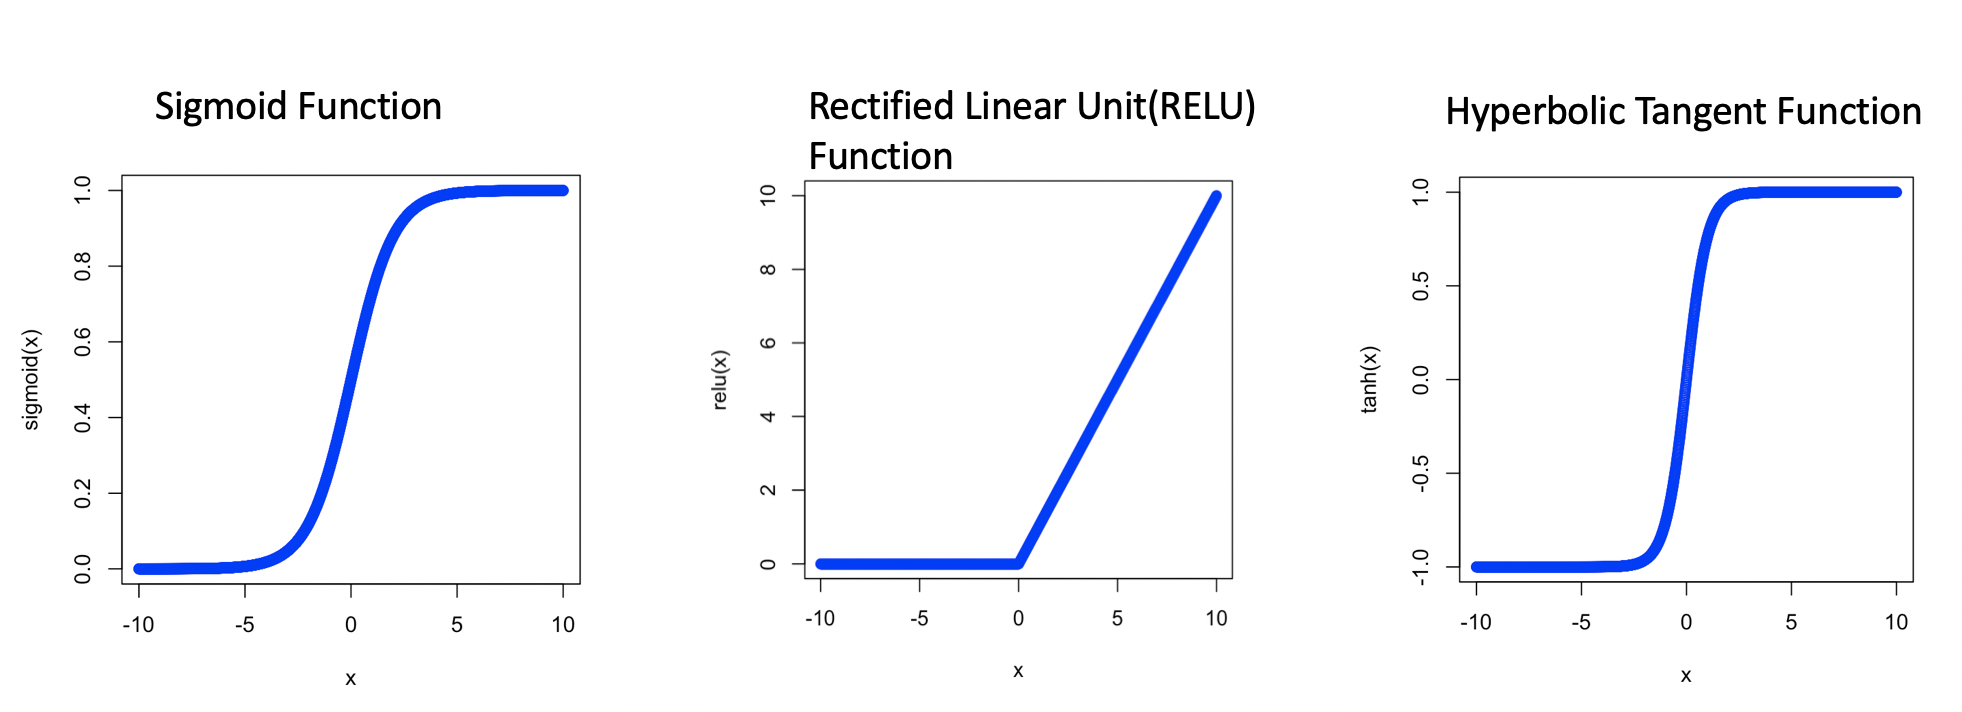
\includegraphics[width=\linewidth, scale=1]{activations.png}
  \caption{Plot of sigmoid, RELU and Tan-h activation functions}
  \label{fig:activations}
\end{figure}
%todo crosscheck  gradient decent function and show more of the chain rule %
To get an accurate estimation of the output, the weights and bias that would achieve this, have to be estimated. One popular algorithm used for this is gradient descent. The gradient descent algorithm aims to minimize this loss. Its steps can be seen below. 
\begin{enumerate}
 \item  Randomly initialize the weights and the bias
 \item Forward propagation, compute $z$ as seen in figure \ref{fig:neuron}, then use $z$  to calculate the expected output using the activation function. 
  \item Using a chosen loss function, $\mathcal{L}(\hat{y},y)$ that compares the expected output and the estimated output, we can calculate the loss.
  \item Calculate the partial derivative of the loss function with respect to the weight, $\frac{\partial \mathcal{L}(\hat{y},y)}{\partial w}$ and the bias, $\frac{\partial \mathcal{L}(\hat{y},y)}{\partial b}$. These partial derivative are arrived at via  backpropagation, which involves using the chain rule. With backpropagation, for example $\frac{\partial \mathcal{L}(\hat{y},y)}{\partial w } = x\frac{\partial \mathcal{L}(\hat{y},y)}{\partial \hat{y} } \frac{\partial \hat{y}}{\partial z }  $  and $\frac{\partial \mathcal{L}(\hat{y},y)}{\partial z} = \frac{\partial \mathcal{L}(\hat{y},y)}{\partial \hat{y} } \frac{\partial \hat{y}}{\partial z }  $.
    \item Update the weight and bias using the below, where $\alpha$ is the learning rate.
\[W = W - \alpha \frac{\partial \mathcal{L}(\hat{y},y)}{\partial W}\]
\[b = b - \alpha \frac{\partial \mathcal{L}(\hat{y},y)}{\partial b}\]
\item Repeat step 2 to 5 till difference of current values and the updated values are at a expected threshold.
\end{enumerate}

Note that the formula $z$ can also be written as $W^TX +b$. Where  $W$  and $X$ are the matrix representation of the input and weights of size, $n \times m $  respectively.  Moreover, $b$ is a $n  \times n$ size vector of the biases.
%more of an explanation
There is a range of loss functions used that are usually linked to an activation function. One loss for binary classification is the log loss which can be written as $ -(y \log{(\hat{y})} + (1-y)\log(1-\hat{y} ))$ when the are two classes and the discrete $ - \sum_{j=1}^{K} y\log{\hat{y}} $ for multi-classification. It is also referred to as cross-entropy loss. Sparse cross-entropy loss is an extension of cross-entropy loss, where the outputs are mutually exclusive.  Meaning each input can only belong to one output class and represent using one-hot embeddings.

When neurons are stacked together, they form a neural network as seen in Figure \ref{fig:neuralnetwork}. This shows a 2 layer network with one hidden layer with three neurons. The output of the activation function of the hidden layer servers as an input to the output layer. Usually, the more complex the problem, the deeper the network.
% maybe find  a diagram of the functionsWhen using gradient decent ,  The RELU function is usually the activation function of choice for hidden layers. This is because the RELE function has  less of an effect when the slope function goes to zero, as seen in \ref{activations}, which allows for faster learning. 


\begin{figure}
\centering
  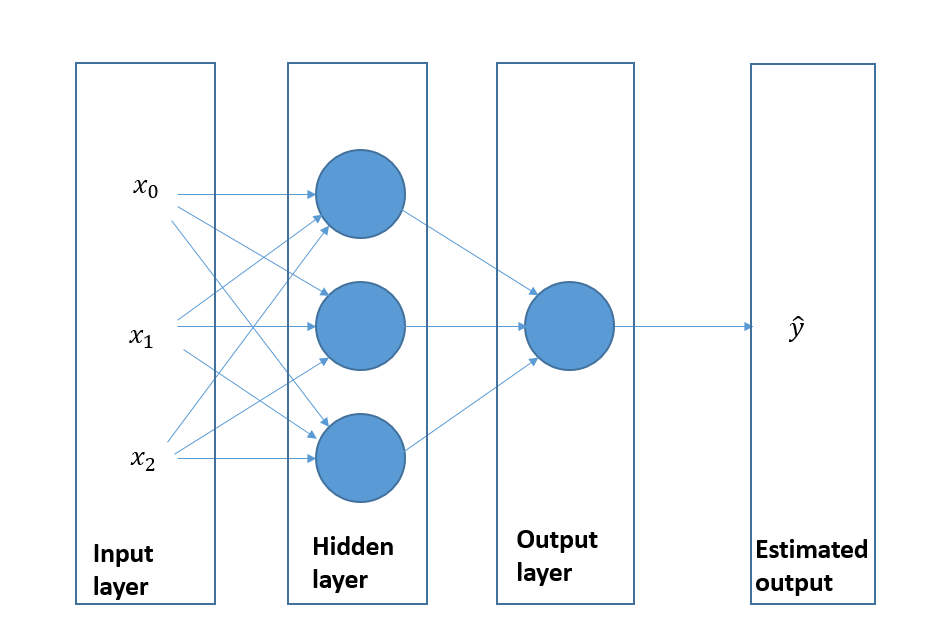
\includegraphics[width=75mm,scale=0.75]{multi-layer-network.PNG}
  \caption{Neural Network structure}
  \label{fig:neuralnetwork}
\end{figure}

\section{Optimization}
% todo find papers for all these regularzation%
The performance of a neural network can be affected by a range of items. This includes the learning rate, the number iterations before the gradient descent algorithm converges, the number of hidden layers, the number of hidden units in each layer and the activation function to name a few.  
These items are referred to as hyperparameters. 

%maybe add dev set%
When evaluating the performance of a neural network, it is best to separate the input data into a training and test set. A standard split of training to test set is about 70%, 30% for a dataset with a size of up to 10000.  The training dataset is used to train the model and arrive at the best possible weights and bias. The test dataset is then used to evaluate the model's performance based on the final parameters, i.e. is the weights and biases. The metric of performance is usually the accuracy which is the percentage of the model's output which was predicted correctly.

When training, it is best to avoid overfitting, i.e. when there is high variance, and the model does better on the training set than on the test set. Underfitting also needs to be avoided. 
Underfitting is when there is a high bias, and the model does not perform well on the training set. 
The usual process is to first combat underfitting by building a model that fits the training data. This can be done by increasing the number of hidden layers or nodes in a hidden layer hence increasing the parameters that fit the data.  Once the train data has been fitted, and the parameters decided, the model is then validated against the test set. If overfitting occurs, the following regularization techniques can be applied to reduce the parameters as listed below:
\begin{itemize}
    \item Dropout - This involves setting a probability at which to drop a percentage of nodes in order to reduce the number of parameters 
    \item Early Stopping -  this involves stopping the training at an early stage. By stopping the training at an early stage, it reduces the size of the parameters learned. 
    \item Data Augmentation - One cause of overfitting is the lack of varied data. Data augmentation is mainly used in the image classification space to reduce the issue of varied data. It involves applying various augmentation techniques such as horizontal flipping, random cropping, to produce a more varied training set. 
\end{itemize}

%Add equations for this%
When dealing with a large dataset, gradient descent can take a long time to process. As it completes one update step over the whole dataset. Various optimization techniques can be used to reduce this time. Some of these include Stochastic gradient descent which works by first shuffling the data, then updating the parameters for each training set. Another is mini batch gradient descent which takes a subset of the data called batches on which the parameters are updated. The batches sizes are usually in factors of 32 because it allows for easier computing. Usually when implementing models, a step is refers to one iteration in which one batch is processed and an epoch  referes to when the whole dataset i.e. all the batches for the dataset has been processed. Other optimizations are RMS prop and Adam optimization, which help with the smoothness of the gradient descent using various hyperparameters and theories such as exponentially weighted averages.
 
Another essential item is normalization; usually, when the input to a neuron is normalized, it tends to train better. In deeper neural networks, there have also been benefits found with normalizing the linear input $z$ to each activation function at every layer. Some of these normalization techniques include local response normalization and batch normalization.



\section{Convolutional Neural networks}
%maybe talk about the flipping%
% also explain stride and give the formula for the parameters and where the features come in
A convolutional neural network is simply a neural network mainly for inputs with a grid structure such as time-series data and particularly images. The network uses a convolution operation in place of matrix multiplication in at least one of its layers as defined in \citep{Goodfellow-et-al-2016}. The convolution operation is typically represented with an asterisk:s  and seen below representing. 
\[ s(t) = (x * w)(t) \] 
where $x$ is the input, and $w$ is the kernel, and the output is usually referred to as the feature map.
\[ s(t) = \int x(a) w(t - a)da \] 
In terms of matrices, it can also be written as the below where $I$ for example is a two-dimensional image and $K$ is the two-dimensional kernel
\[S(i, j) = (I*K)(i, j) = \sum_m \sum_nI(m, n)K(i- m, j- n). \]
Convolutional networks also include a pooling layer which applies a function that replaces an input with a summary statistic of the nearby inputs, sometimes reducing the input matrix size.

By applying specific kernels to input, in the case of image recognition, a layer can learn specific features of the image such as edge detection for example. When applying a  kernel to an input, the output is usually reduced as seen in figure \ref{fig:convolution}. With the reduced output in order to prevent a shrinking output as we go deeper into a network and to hold more information on the image, padding can be applied. Padding involves adding a border containing $p$  pixels to the image.  This leads to an increase in the output size as a kernel is applied. Another essential term, in convolutional neural networks, is stride. Stride involves taking  $s$ steps for the element-wise multiplication with the kernel, rather than 1 step. When a kernel of $f \times f$  is applied to an image of  $n \times n $  with a stride of $s$ and a padding  $p$,  the resulting output size is given by the equation 

    
\[ \left[ \frac{n + 2p -f }{s} +1 \right]   \times  \left[ \frac{n + 2p -f }{s} +1 \right]
\]

Convolutional neural networks can also take in a volume input by simply be extending the kernels over the dimensions of the input.  


\begin{figure}
\centering
  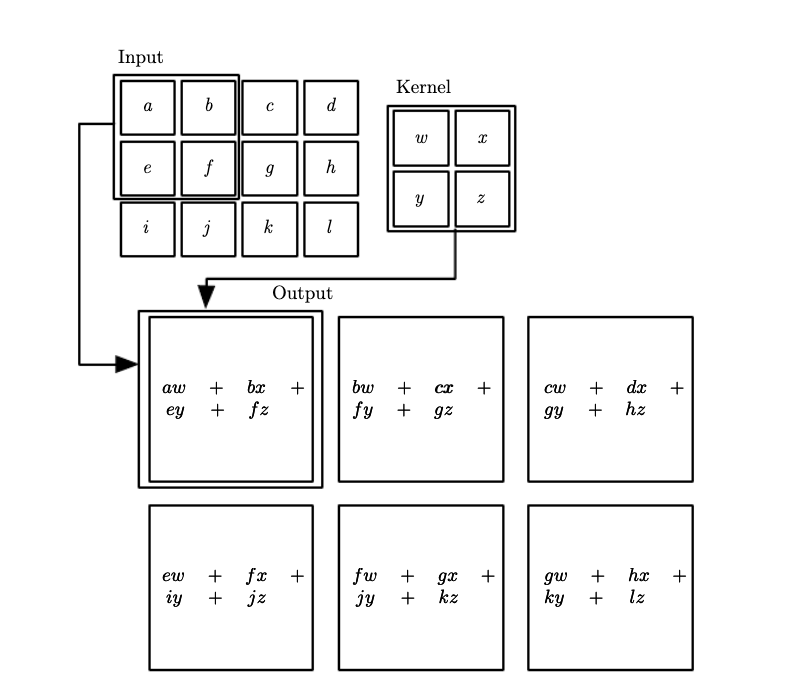
\includegraphics[width=75mm,scale=0.75]{convolution.png}
  \caption{Convolution operation without flippings sourced from \citep{Goodfellow-et-al-2016}}
  \label{fig:convolution}
\end{figure}






